% !TeX spellcheck = it_IT

\documentclass[12pt]{report}
\usepackage[a4paper,top=3cm,bottom=3cm,outer=3.07cm,inner=3.07cm,verbose,heightrounded]{geometry}

\usepackage[english,italian]{babel}
\usepackage{tikz}
\usepackage{pgfplots}
\usepackage{pgfplotstable}
\pgfplotsset{
	compat=newest,
	every tick label/.append style={font=\scriptsize},
	every node near coord/.append style={font=\scriptsize,color=black}
}
\usepgfplotslibrary{ternary}
\usetikzlibrary{calc}
\usepackage{float}
\usepackage{listings}
\usepackage{color}
\lstset{
	frame=tb,
	aboveskip=3mm,
	belowskip=3mm,
	showstringspaces=false,
	columns=flexible,
	basicstyle={\footnotesize\ttfamily},
	breaklines=true,
	keywordstyle=\color{blue},
	commentstyle=\color{gray},
	stringstyle=\color{orange},
	tabsize=2
}
\usepackage[font={small}]{caption}
\usepackage[export]{adjustbox}
\usepackage{pdflscape}
\usepackage{lipsum}

\begin{document}
	\sloppy
	\setlength{\parskip}{10pt}
	\setlength{\parindent}{0pt}
	
	\chapter{Test per la stampa}
	Questa pagina è completamente in bianco e nero.

	\lipsum[1-4]
	\begin{figure}[H]
		\centering
		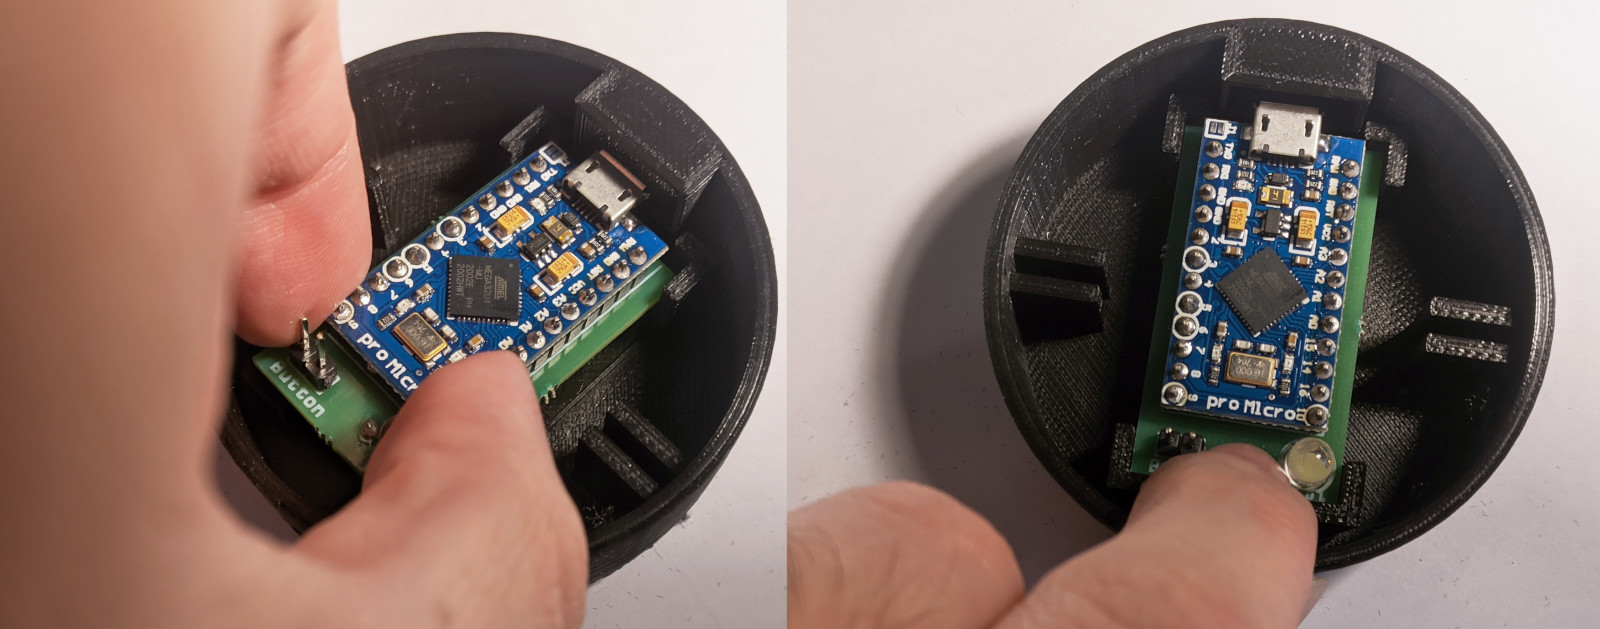
\includegraphics[width=\textwidth]{Dispositivo_files/assembly_14.jpg}
		\caption{Esempio di fotografia}
		\label{fig:photo1}
	\end{figure}
	\begin{figure}[H]
		\centering
		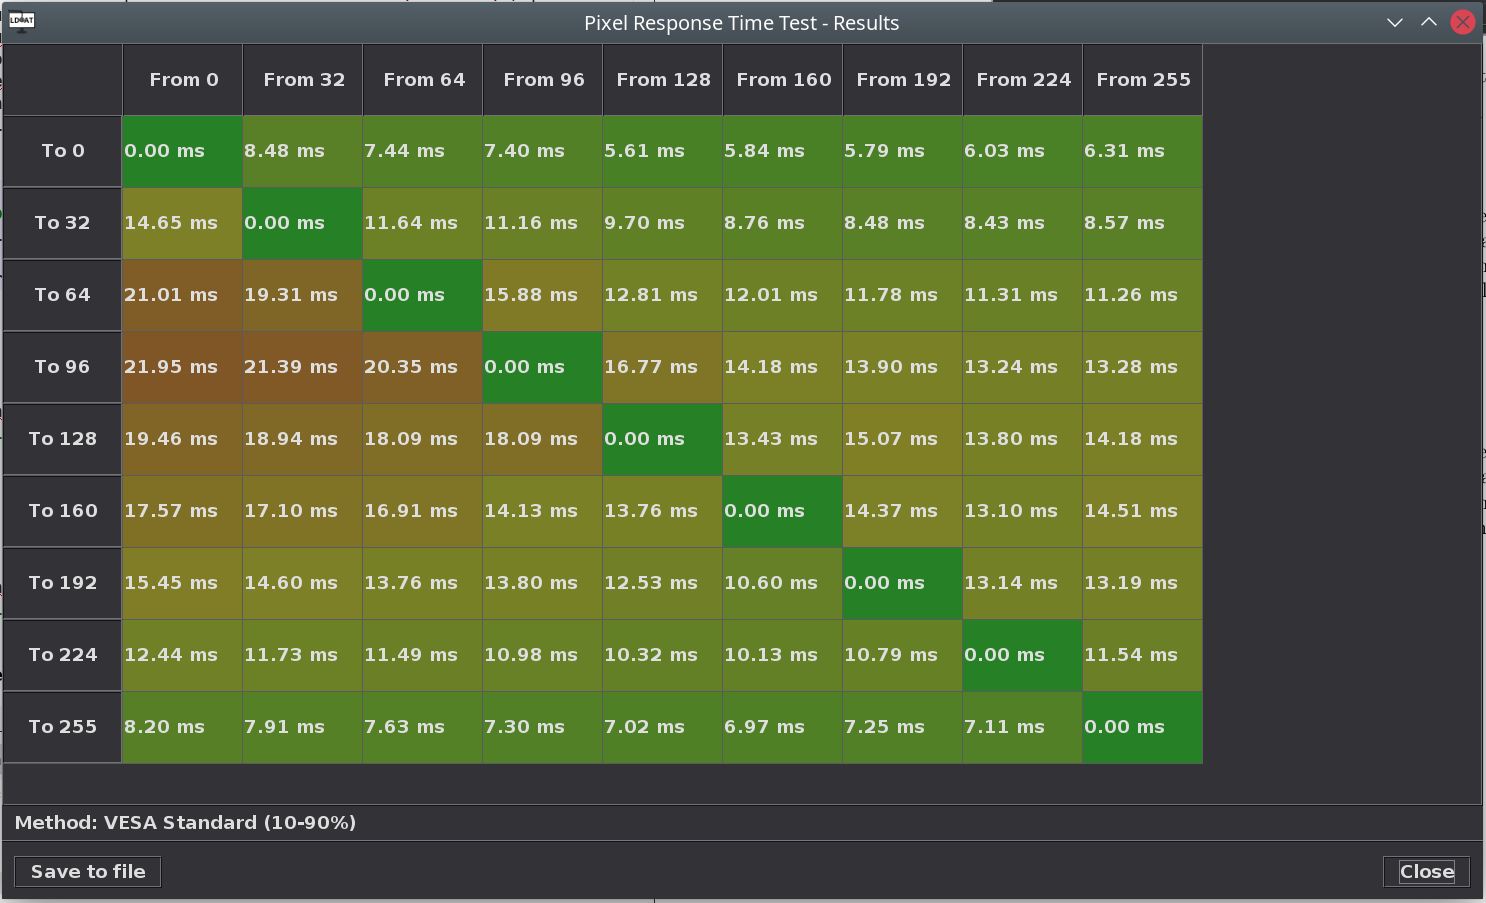
\includegraphics[width=\textwidth]{Applicazione_files/gui_pixelresponse_results.png}
		\caption{I colori rosso e verde devono essere ben distinguibili e il testo deve essere leggibile}
		\label{fig:screen1}
	\end{figure}
	\begin{figure}[H]
		\centering
		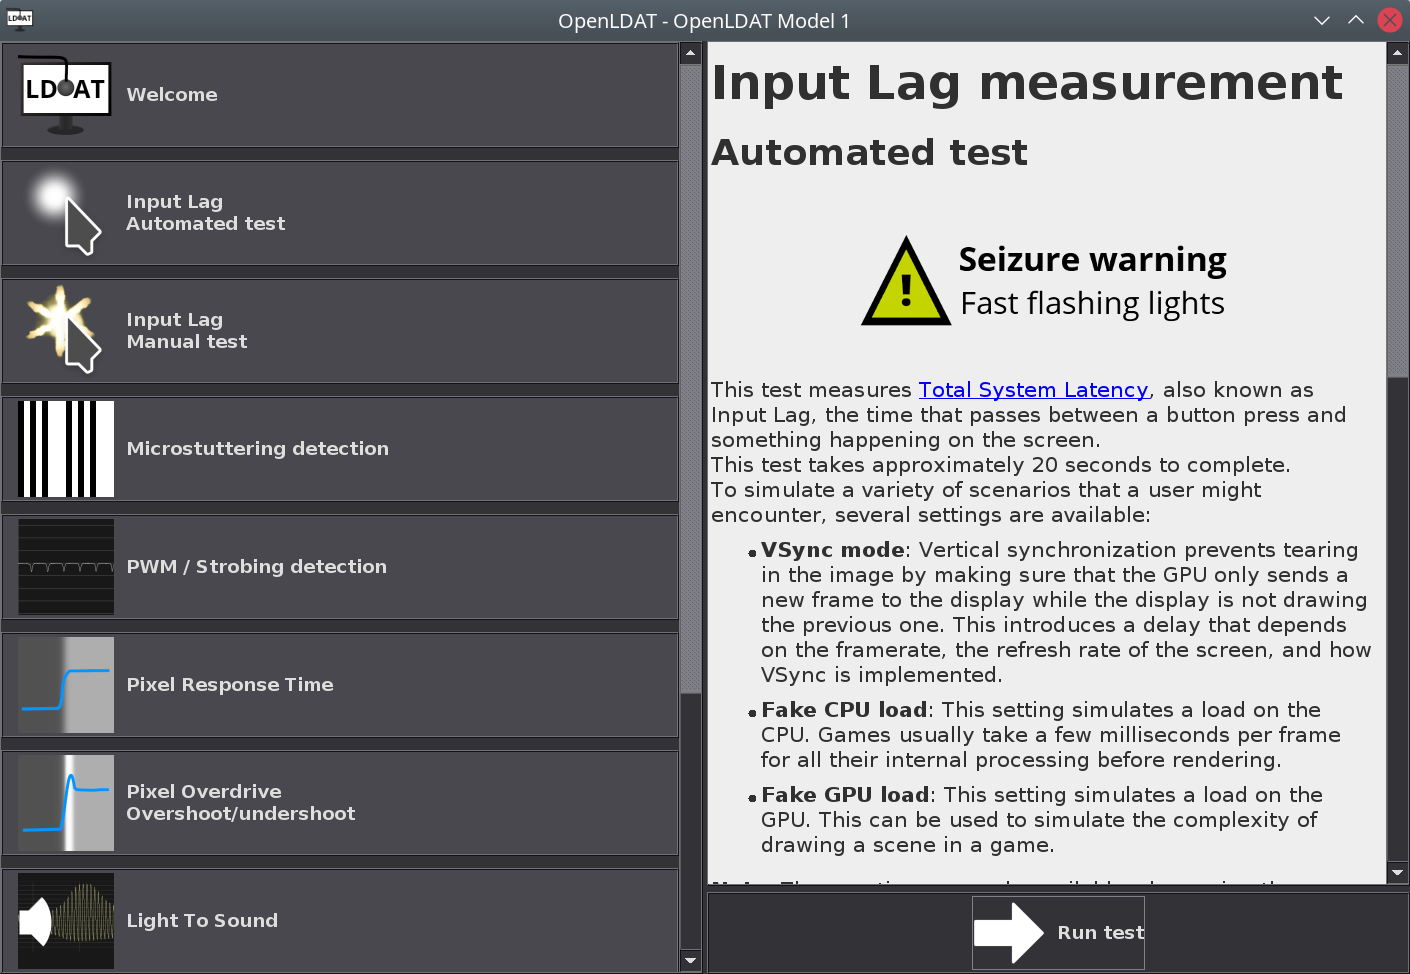
\includegraphics[width=\textwidth]{Applicazione_files/gui_mainMenu2.png}
		\caption{Il testo deve essere leggibile da entrambe le parti}
		\label{fig:screen2}
	\end{figure}
	\begin{figure}[H]
		\centering
		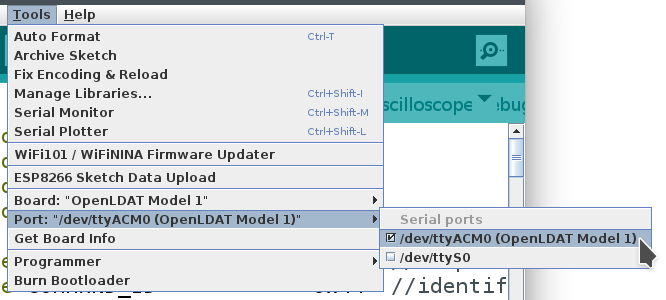
\includegraphics[width=0.7\textwidth]{Dispositivo_files/flashing_03.png}
		\caption{Screenshot chiaro}
		\label{fig:screen3}
	\end{figure}
	\lipsum[5]
	\begin{landscape}
		\centering Questa pagina è in orizzontale e in bianco e nero.
		
		\begin{table}[H]
			\centering
			\adjustbox{max width=\columnwidth}{\begin{tabular}{|l|c|c|c|c|c|c|} 
				\hline
				\textbf{Dispositivo} & \textbf{Tipo} & \textbf{Anno} & \textbf{Refresh} & \textbf{Tecnologia} & \textbf{Retroilluminazione} & \textbf{Testato da}  \\ 
				\hline
				Acer Predator XB271HU & Monitor & 2019 & 165Hz VRR & TN  & Edge LED & Terzi \\ \hline
				Acer Swift 3 & Laptop & 2020 & 60Hz & IPS & Edge LED & Autore \\ \hline
				AOC Q2770P & Monitor & 2014 & 60Hz & IPS & Edge LED & Autore \\ \hline
				ASUS VP228HE & Monitor & 2019 & 60Hz & TN & Edge LED & Terzi \\ \hline
				ASUS VW228 & Monitor & 2011 & 60Hz & TN & Edge LED & Terzi \\ \hline
				BenQ GL2706PQ & Monitor & 2014 & 60Hz & TN & Edge LED & Terzi \\ \hline
				BenQ XL2420T & Monitor & 2012 & 120Hz & TN & Edge LED & Terzi \\ \hline
				Huawei MateBook D & Laptop & 2019 & 60Hz & IPS & Edge LED & Terzi \\ \hline
				iPhone 6S & Smartphone & 2015 & 60Hz & IPS & Edge LED & Terzi \\ \hline
				LG 27GL850-B & Monitor & 2018 & 144Hz VRR & IPS HDR & Edge LED & Terzi \\ \hline
				LG E2360 & Monitor & 2012 & 60Hz & TN & Edge LED & Terzi \\ \hline
				MacBook Pro 13" & Laptop & 2017 & 60Hz & IPS & Edge LED & Terzi \\ \hline
				Octigen M19W & Monitor & 2008 & 60Hz & TN & CCFL & Autore \\ \hline
				OnePlus 3T & Smartphone & 2016 & 60Hz & AMOLED & N/A & Autore \\ \hline
				OnePlus 7 Pro & Smartphone & 2019 & 90Hz VRR & AMOLED & N/A & Terzi \\ \hline
				Philips 32PFS4132 & TV & 2020 & 60Hz & TN & Edge LED & Autore \\ \hline
				Philips 105MB & Monitor & 1997 & N/A & CRT & N/A & Autore \\ \hline
				Samsung C34H890 & Monitor & 2019 & 100Hz VRR & VA & LED Array & Terzi \\ \hline
				Samsung P2770HD & TV & 2011 & 60Hz & TN & Edge LED & Autore \\ \hline
				Sony VAIO SVF1532C5E & Laptop & 2014 & 60Hz & TN & Edge LED & Terzi \\ \hline
				Sharp Aquos LC-40FG3242E & TV & 2020 & 60Hz & TN & Edge LED & Autore \\ \hline
				Thinkpad T480 & Laptop & 2018 & 60Hz & IPS & Edge LED & Autore \\ \hline
			\end{tabular}}
			\caption{\label{tab:display_list}Lista completa dei dispositivi testati}
		\end{table}
	\end{landscape}
	\begin{figure}[H]
		\centering
		\begin{tikzpicture}
			\begin{axis}[name=Segnale, xmin=0,xmax=0.5,ymin=0,ymax=1023,width=.6\textwidth,xlabel=Tempo (s),ylabel=Valore,xticklabel style={/pgf/number format/fixed}]
				\addplot[lightgray] file{Applicazione_files/pixelOverdriveTest_example_pwm.txt};
				\addplot[red] file{Applicazione_files/pixelOverdriveTest_example_phf.txt};
			\end{axis}
		\end{tikzpicture}
		\caption{Il grigio deve essere distinguibile dal nero degli assi, il rosso deve essere visibile}
		\label{fig:chart1}
	\end{figure}
	\begin{figure}[H]
		\centering
		\pgfplotstableread[col sep=comma]{
			model,odoff,odoffemin,odoffemax,odon,odonemin,odonemax,fix
			Riga 1,NaN,NaN,NaN,2.61,1.48,3.80,-10
			Riga 2,NaN,NaN,NaN,4.06,2.79,3.76,-10
			Riga 3,4.80,3.39,11.83,NaN,NaN,NaN,-10
			Riga 4,7.81,5.17,27.90,7.79,4.26,18.25,-10
			Riga 5,NaN,NaN,NaN,8.44,5.71,20.67,-10
			Riga 6,12.33,6.06,9.01,7.37,3.09,3.74,-10
		}\dataset
		\begin{tikzpicture}
			\begin{axis}[xbar, bar width=8pt, y dir=reverse, ytick=data, yticklabels from table={\dataset}{model}, yticklabel style={align=right}, table/y expr = \coordindex, nodes near coords, reverse legend, xlabel=Tempo (ms), width=0.7\textwidth, height=7.5cm, xmin=0, ymin=-1, ymax=6] %ymax messo a mano con il numero di display per migliore formattazione
				\addplot plot[forget plot] table[x=fix] {\dataset};
				\addplot plot [error bars/.cd, x dir = both, x explicit] table[x=odoff, x error plus=odoffemax, x error minus=odoffemin] {\dataset};
				\addplot plot [error bars/.cd, x dir = both, x explicit] table[x=odon, x error plus=odonemax, x error minus=odonemin] {\dataset};
				\legend{Barra B,Barra A}
			\end{axis}
		\end{tikzpicture}
		\caption{I valori devono essere leggibili}
		\label{fig:chart2}
	\end{figure}	
	Il seguente listato è colorato, deve essere leggibile.
	\lstinputlisting[language=Java]{Applicazione_files/DeviceExample.java}
	
	Questo conclude il test di stampa. Grazie!
	
\end{document}
